\title{Implementation of Integral LQG Control for AUV Depth Tracking}
\author{Joseph Gland}
\documentclass{article}
\usepackage{graphicx}%needed for images
\usepackage{amsmath}%needed for bmatrix and operatorname
\begin{document}

\maketitle

\begin{center}
\Huge 
DRAFT
\normalsize
\end{center}
\vspace{0.5cm}

Depth control for an AUV can be achieved in many ways, but is often neither obvious nor intuitive as all states of the system are not directly measurable.  The situation is further complicated as many people assume depth control to be simple when design objectives like tracking control (as opposed to just regulation control) and disturbance rejection require some advanced techniques.  First, consider the free body diagram for a rigid body in viscous fluid (such as water) shown in Figure \ref{fig:freeBody}.  Note that the depth datum has been set at the fluid surface with the downward direction chosen to be positive.

\begin{figure}[h]
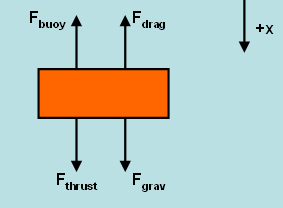
\includegraphics[width=0.5\textwidth]{FreeBodyDiagram.png}
\centering
\caption{Free body diagram for a rigid body suspended in viscous fluid}\label{fig:freeBody}
\end{figure}

The free body diagram shows a total of four forces acting on the vehicle: 
\begin{itemize}
\item $F_{grav}$ is the gravitational force acting on the vehicle.  It is constant and can be determined via $F_{grav}=mg$ where $g$ is the gravitational constant near the surface of the earth.
\item $F_{thrust}$ is the force applied to the vehicle by the onboard thrusters.  The thrusters are of course controlled by the vehicle's computer and are our only means of exerting control authority on the system.
\item $F_{buoy}$ is the buoyant force on the vehicle.  Like gravitational force, it is constant and is computed via the relation $F_{buoy}=\rho_{water}V_{sub}g$ where $\rho_{water}$ is the density of water, $V$ is the displaced volume of the AUV (constant for a rigid sub), and $g$ again is the gravitational constant near the surface of the earth.
\item $F_{drag}$ is the drag on the vehicle due to motion in a viscous medium.  A linear model for drag is $F_{drag}=c\dot{x}$, where $c$ is a drag parameter for the vehicle and $\dot{x}$ is the vehicle's velocity.  A more accurate model of drag is $F_{drag}=\operatorname{sgn}(x)c\dot{x}^{2}$, but it is nonlinear and is therefor hard to incorporate with linear control theory.  We will assume the former drag model in this document, and postpone use of the later nonlinear drag model for a more advanced controller.
\end{itemize}
The above forces can be applied to a single equation of motion using Newton's law:  
\begin{equation}
\label{eq:newton1}
m\ddot{x}=\sum_{i}F_i=F_{grav}+F_{thrust}-F_{buoy}-F_{drag}
\end{equation}
where $m$ and $\ddot{x}$ are the mass and acceleration of the vehicle, respectively.  By substituting in the relation for $F_{drag}$, replacing the $F_{thrust}$ variable with the control input variable $u$, renaming the sum of the constant terms $F_{grav}-F_{buoy}=d_0$, and dividing through by $m$, equation \ref{eq:newton1} can be rewritten as:
\begin{equation}
\ddot{x}=-\frac{c}{m}\dot{x}+\frac{1}{m}u+\frac{1}{m}d_0
\end{equation}
By setting $x_1=x$ and $x_2=\dot{x}$, the system's state space form is:
\begin{equation*}%don't number this equation
\begin{bmatrix} \dot{x_1} \\ \dot{x_2} \end{bmatrix}=\begin{bmatrix} 0 & 1 \\ 0 & -\frac{c}{m} \end{bmatrix} \begin{bmatrix} x_1 \\ x_2 \end{bmatrix} + \begin{bmatrix} 0 \\ \frac{1}{m} \end{bmatrix}u + \begin{bmatrix} 0 \\ \frac{1}{m} \end{bmatrix}d_0
\end{equation*}
or, more succinctly using symbols for vectors and matrices:
\begin{equation}
\label{eq:system}
\pmb{\dot{x}}=A\pmb{x}+Bu+B_0d_0
\end{equation}
This dynamical model is surprisingly simple.  The only two unknowns are $m$ and $c$, which are the mass and drag coefficient of the vehicle respectively.  Vehicle mass $m$ is very straightforward to measure and can be done with relatively good precision.  The drag coefficient is more difficult to determine; it can be modeled analytically or determined experimentally.  It is difficult to determine an analytical model since the model depends on the exact shape of the vehicle.  Experimentally, the sub can be released from rest in water and its unforced response can be analyzed to solve for its drag parameter.  

Assuming our sensing hardware only provides us with a noisy measure of depth, our measurement equation for the system can be written as:

\begin{equation}
\begin{split}
\label{eq:measurement}
y&=\begin{bmatrix} 1 & 0 \end{bmatrix} \begin{bmatrix} x_1 \\ x_2 \end{bmatrix} + n \\
&=C\pmb{x}+n
\end{split}
\end{equation}
where $n$ is a random white noise variable with intensity $N$.  The white noise variable is a simple model for a sensor with noise.  While other noise models exist, this model is simple to generate as the intensity $N$ can be roughly approximated from simple experimentation.  The model also fits well into our design framework later on.

We have now generated a model for an AUV for depth control.  Note that the system, described by equations \ref{eq:system} and \ref{eq:measurement}, is both linear and time-invariant.  The system model is controllable and observable as well, which allows us to apply a number of powerful control theory tools.

Note that at this point, if our measurement equation was simply $\pmb{y}_{full}=\begin{bmatrix} 1 & 0 \\ 0 & 1 \end{bmatrix} \pmb{x}$ we could immediately implement the full state feedback control $u=-K\pmb{x}=-K\pmb{y}_{full}$.  Then we would just have to design $K$ to meet our control design objectives.  Unfortunately, our measurement equation is instead equation \ref{eq:measurement} which implies that $\pmb{x}\neq y$.

If we can't implement $u=-K\pmb{x}$ for full state feedback, the concept of certainty equivalence can be used \emph{for linear time-invariant systems}.  The certainty equivalence principle suggests that instead of using $u=-K\pmb{x}$, we can implement $u=-K\pmb{\hat{x}}$ where $\pmb{\hat{x}}$ is the output of an observer.  This concept works well for linear time-invariant systems; however, it can fail spectacularly for time-varying and/or nonlinear systems.

There are many ways of estimating $\pmb{\hat{x}}$.  Assuming we have a reasonably accurate model for the system dynamics, a Luenberger observer can be used to estimate the system states.  A Luenberger observer, shown in equation \ref{eq:luenberger}, uses a copy of the model of the system along with a correction term to continually predict system states.  If we neglect the constant term $d_0$ in equation \ref{eq:system}, then we can estimate the states of the system with:
\begin{equation}
\begin{split}
\label{eq:luenberger}
\pmb{\dot{\hat{x}}}&=A\pmb{\hat{x}}+Bu+L(y-\hat{y}) \\
\hat{y}&=C\pmb{\hat{x}}
\end{split}
\end{equation}
where $L$ is the observer gain matrix which is to be appropriately designed.  

One common way of designing the observer gain matrix is to directly place the observer poles. The larger in magnitude the observer poles are, the faster the observer's state estimate will converge to the actual state.  If the observer poles are too large in magnitude, however, the observer can become numerically unstable.  In practice observer poles are typically chosen to all be real, negative, and at least five times greater in magnitude than the largest pole of $[A-BK]$.  For our system, if we had a vector of desired observer poles $\pmb{\mu}$, MATLAB could generate the appropriate gain matrix $L$ using the command \verb+L=(place(A',C',mu))'+.

A more sophisticated way of designing the observer gain matrix is to solve the filter algebraic Riccati equation.  With our model of the noise acting on the sensor, we can solve the Riccati equation.  The solution for $L$, when incorporated into a Luenberger, is actually the simplified steady-state version of the celebrated Kalman filter.  The MATLAB incantation \verb+L=lqe(A,C,B_0,zeros(2),N)+ solves the Riccati equation and produces the stochastically optimal gain matrix $L$.  The zero matrix is used because we are assuming there are no random forces are acting on the vehicle.

We now have two different methods to design $L$.  The observer can now be used to generate $\pmb{\hat{x}}$ which is an estimate of the true states $\pmb{x}$ using only measurements $y$.  The Luenberger observer, in equations \ref{eq:luenberger}, can be incorporated into our system software and integrated over time.  If our measurements $y$ are made at a known fixed interval, we can implement a discrete version of equations \ref{eq:luenberger} with MATLAB.  The initial estimate $\pmb{\hat{x}}$ can be set to any physical state the system could actually achieve; however, the further off the initial estimate is the longer it will take for the estimates to converge to the true state.   

%
% DO I HAVE MY MATLAB SYNTAX RIGHT for lqe()?
%
%      ***********
%     *           * 
%     *   *   *   *
%     *           *  <- blockhead
%     *  _______  *
%     *           *
%      ***********
%

Now that we have an estimate for all our states, we can use the certainty equivalence principle to incorporate the full state feedback control law: 
\begin{equation}
\label{eq:equivalencePrinciple}
u=-K\pmb{\hat{x}} 
\end{equation}
which will regulate the system states to zero (we'll worry about tracking control later).  Of course we still have yet to design the matrix $K$.  There are conflicting criteria for the design of $K$ similar to the criteria for the design of $L$.  The $K$ matrix can be designed exclusively by placement of the controller poles (ie the poles of $[A-BK]$).  We typically want these poles to be real (to minimize oscillatory system response) and negative (to have a stable system).  The greater in magnitude these poles are, the faster the system will respond which is very desirable.  Unfortunately, the faster the system responds, the larger the control output has to be.  In the real world, this means that larger magnitude controller poles will require the thrusters to push harder.  At worst this could directly saturate the thrusters and the vehicle could go unstable, at best the thrust required to keep the vehicle at depth might prevent the thrusters from being able to be used by other controllers (perhaps controllers that are trying to keep the vehicle oriented correctly).  The method of directly placing the controller poles can be an effective method with lots of simulation and experimentation.  MATLAB of course has a handy command for the design of $K$ given a vector of controller poles $\pmb{\mu}$.  In fact, it is the intended use for a command we used previously: \verb+K=place(A,B,mu)+.

While the pole placement method for $K$ works, it requires numerous simulation and experimental work in order to find controller poles that make the system fast enough while preventing the system from using its thrusters too much.  The LQR algorithm (an acronym for Linear Quadratic Regulator) attempts to formalize this design tradeoff and simplify the design of $K$.  The design method actually minimizes the cost function $J=\frac{1}{2}\int_{0}^{\infty}\{\pmb{x}^TQ\pmb{x}+uRu\}dt$ where $Q$ and $R$ act as weighting matrices for different design objectives.  The $Q$ matrix penalizes the error between the system states and zero, so a large $Q$ would wind up designing a control matrix $K$ with large values, exert large thrusts, and make the system respond very quickly.  The $R$ matrix (a scalar for our problem since we only have one control output) penalizes control signals, so a large $R$ would wind up designing a control matrix $K$ with small values, exert small thrusts, and make the system respond very slowly.  With appropriate choice of $Q$ and $R$, we can selectively choose to ``worry'' more about some states more than others or some states more than the control outputs.  MATLAB's routine for solving for $K$ given $Q$ and $R$ is \verb+K=lqr(A,B,Q,R)+.  With this method, we still have to simulate how the system will respond for various conditions, but the design methodology is much faster and easier to use.  In the long run, it winds up being much easier and more intuitive to tweak the $Q$ and $R$ matrices than it is to tweak the controller poles (ie the poles of $[A-BK]$).

The use of the simplified steady-state Kalman filter for the design of $L$ along with the use of the LQR for the design of $K$ is called a Linear Quadratic Gaussian controller, or LQG for short.  The Gaussian part of the name comes from the steady-state Kalman filter, which makes an assumption that all noise sources can be treated as Gaussian random variables (we skipped over the derivation of this and just used MATLAB to give us a solution).  By using our $L$ designed by MATLAB's \verb+lqe()+ command and our $K$ designed by MATLAB's \verb+lqr()+ command in equations \ref{eq:luenberger} and \ref{eq:equivalencePrinciple}, we can implement the controller block in the Figure \ref{fig:LQGBlockDiagram} which almost completes the design of our depth control system.

\begin{figure}[h]
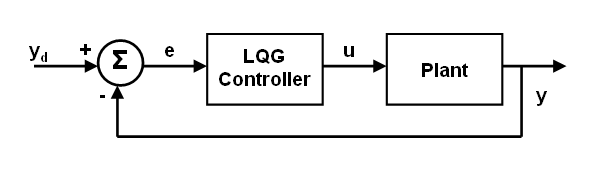
\includegraphics[width=0.8\textwidth]{LQGBlockDiagram.png}
\centering
\caption{Block Diagram for an LQG controller.  A strict LQG controller only allows the input $\pmb{y_d}=0$.  The Ad Hoc LQG Servo controller is implemented by simply setting $\pmb{y_d}=$constant, but is not recommended.}
\label{fig:LQGBlockDiagram}
\end{figure}

We now have a full LQG controller.  We could stop right here and the controller would reliably regulate the depth of the AUV to zero under the assumption that there are no constant disturbances acting on the vehicle (ie assuming that $F_{grav}-F_{buoy}=d_0=0$).  The constant disturbance model, however, is in general not zero.  In fact, competition rules requires that the vehicle is positively buoyant, so $F_{grav}-F_{buoy}=d_0<0$.  Also, we will definitely want to be able to go to depths other than zero.

\begin{figure}[h]
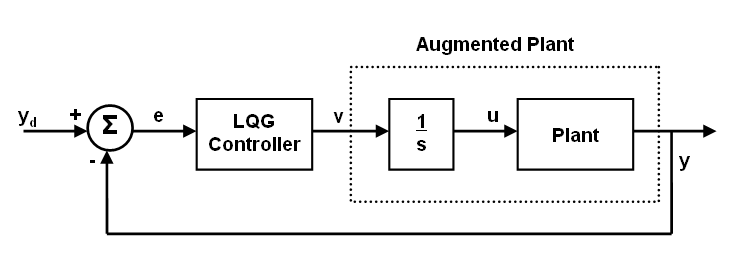
\includegraphics[width=0.8\textwidth]{LQGAugmentedPlant.png}
\centering
\caption{Augmented plant}
\label{fig:LQGAugmentedPlant}
\end{figure}

\begin{figure}[h]
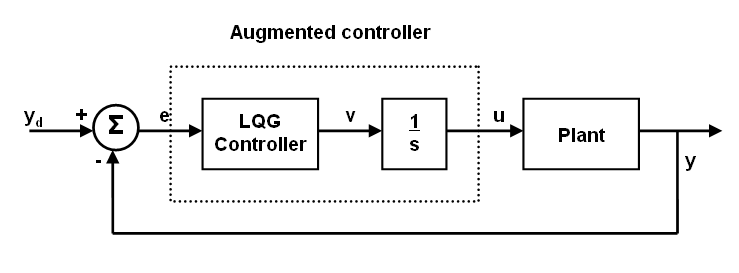
\includegraphics[width=0.8\textwidth]{LQGAugmentedController.png}
\centering
\caption{Augmented Controller}
\label{fig:LQGBlockDiagram}
\end{figure}

\begin{figure}[h]
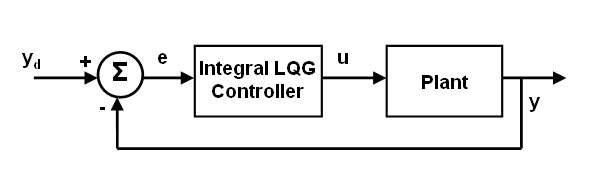
\includegraphics[width=0.8\textwidth]{LQGIntegralController.png}
\centering
\caption{Augmented Controller}
\label{fig:LQGBlockDiagram}
\end{figure}

\end{document}